
The contribution of this study on travel mode choice is the research on modeling choices in travel mode selection using game theory concepts, and using an evolutionary analysis to determine the behavior of the travelers.
\clearpage

\section{Evolutionary Game Theory and Travel Mode Choice}
Evolutionary game theory is used in this paper as a vehicle for discussing travel mode choice based on the following apparent similarities: 
\paragraph{}A group can be a substitute for an individual as a participant in evolutionary game theory, and the proportions of the individuals choosing different pure strategies in the group can substitute for mixed strategy. The results of travel mode choice are group behavior within the travel mode subsystems, and the only proportions of individuals choosing each travel mode are meaningful for management and study.
\paragraph{}Group Nash equilibrium means that the frequency of the adopted strategies makes the strategy payoffs exactly equal with no one desiring a change in strategy, then the percentage of individuals choosing each different strategy remains stable and reaches equilibrium. In the stable travel context, a travel mode choice will tend to be stable, the Nash equilibrium of the evolutionary game will be changed by the means of traffic control, the construction, and the structure of the transportation system.
\paragraph{}The nature of group strategies acts is that only a bounded rationality human gets closer to Nash equilibrium by summarizing their experience and adjusting their strategies rather than by using a perfectly rational method and Nash equilibrium analysis as reasoning. The players can obtain information such as travel time, travel cost, and traffic information, and they can observe the historical results and the strategies adopted by others. The inhabitants observe and experience the service provided by trip modes during their frequent travels and finally determine their strategies. Although they are bounded by rationality, constantly repeated travel leads the structure of travel mode choice by modes to reach excellent stability.
\subsection{Evolutionary Game Model}
The extensive form of the sequential, the game displayed in Figure 1, describes the process of travel mode choice. Two conditions have been implemented in this model.
\begin{itemize}
\item Travelers can be divided into two main categories: car owners and noncar owners. As mentioned before, travel is a two stage process, first, every player chooses whether they own a car or not; then, the car owners will select from one of four modes: car, taxi, bus, or rail, and the noncar owners will only select from taxi, bus, or rail.
\item The payoff function that inhabitants must contribute is independent of the proportion of inhabitants traveling in a particular mode.

\end{itemize}
\paragraph{} As mentioned in Chapter 1, the extensive form is defined by three  main objects.
\begin{itemize}
\item the set of players $N = {1,...,n}$, all travelers are players.
\item The strategy sets of the players are $S_1 = {Car owneer, Noncar owner}$ and ${S_2 = {Travel by car, Travel by taxi, Travel by bus, Travel by rail}}$.
\item The payoff functions of the players are $f_{car} = u_1$, $f_{taxi} = u_2$, $f_{bus} = u_3$, and $f_{rail} = u_4$
\end{itemize}
\paragraph{}Players use mixed strategy, because it is impossible for them to travel using the same pure strategy mode multiple times with certainty.
\paragraph{}As explained in Chapter 1, the mixed strategy happens when an individual plays one of the pure strategies of a game with a continuous probability $p$ between 0 and 1. As a result, the payoff the of the individual using mixed strategy depends on the probabilities of the mixed strategy.
\paragraph{}Figure 3.1 shows the game model of travel mode choice, we note that in stage 1 of the game $p_c$ and $p_n$ are the probabilities of car owners and non car owners respectively. In stage 2, $p^c_{c}$, $p^{c}_{t}$, $p^c_{b}$, and $p^c_{r}$ are the respective probabilities of car owner traveling by car, taxi, bus or rail. The probabilities of the noncar owner traveling by taxi, bus or rail are $p^n_{t}$, $p^n_{b}$, and $p^n_{r}$.
\paragraph{}The payoff function of the players are the following: 
\begin{equation}
f_{car} = T_{car} C_{car}
\end{equation}
\begin{equation}
f_{taxi} = T_{taxi} C_{taxi}
\end{equation}
\begin{equation}
f_{bus} = T_{bus} C_{bus}
\end{equation}
\begin{equation}
f_{rail} = T_{rail} C_{rail}
\end{equation}
\paragraph{}where travel time averages for car, taxi, bus, and rail are $T_{car}$, $T_{taxi}$, $T_{bus}$, $T_{rail}$, and their average travel costs are $C_{car}$, $C_{taxi}$, $C_{bus}$, $C_{rail}$ respectively.
\begin{figure}
 
  \centering
  \begin{tikzpicture}[baseline] % baseline makes the example number stay at the top of the tree
   \Tree[.N [.\textit{Car Owner} [.Car \textit{$U_1$} ][.Taxi \textit{$U_2$} ][.Bus \textit{$U_3$} ][.Rail \textit{$U_4$} ]][.\textit{Non Car Owner} [.Taxi \textit{$U_2$} ][.Bus \textit{$U_3$} ][.Rail \textit{$U_4$} ]]]
     \end{tikzpicture}%
  \caption{Travel mode choice game\label{fig:2}}
\end{figure}
\subsection{Nash Equilibrium of Travel Mode Choice Game}
According to the Folk Theorem mentioned in Chapter 1, any payoff vector satisfying individual rationality can be obtained through a set of specific subgame perfect equilibriums in an infinitely repeated game. Tn travel mode choice, there are two subgame: Car owner subgame and noncar owner subgame, as shown in figure \ref{fig:2}. If Nash equilibrium is reached in each of the subgames, the Nash equilibrium of the game is subgame perfect Nash equilibrium. As mentioned in the previous section, backward induction is the solution method for obtaining the Nash equilibrium of this game.
\begin{figure}
  \centering
  \begin{tikzpicture}[baseline] % baseline makes the example number stay at the top of the tree
   \Tree[.\textit{Car Owner} [.Car \textit{$U_1$} ][.Taxi \textit{$U_2$} ][.Bus \textit{$U_3$} ][.Rail \textit{$U_4$} ]]
     \end{tikzpicture}%
  \caption{Car owner subgame\label{fig:3}}
\end{figure}
\subsubsection{Nash Equilibrium of Car Owner Subgame}The key feature of mixed strategy Nash equilibrium is that the expectations of the pure strategies are equal, that is, in car owner subgame of figure \ref{fig:3}, the products of the travel mode's payoffs and its probabilities are equal and the sum of their probabilities is 1, so that 

\begin{equation}\label{eq:8}
\mu_1 r^c_{c} = \mu_2 r^{c}_{t} = \mu_3 r^c_{b} = \mu_4 r^c_{r}
\end{equation}
\begin{equation}\label{eq:9}
\mu_1 r^c_{c} +  \mu_2 r^{c}_{t} + \mu_3 r^c_{b} + \mu_4 r^c_{r} = 1
\end{equation}

Solving \ref{eq:8} and \ref{eq:9}
\begin{equation}\label{eq:5555}
r^c_{c} = \frac{1}{1+ (\mu_1 / \mu_2)+(\mu_1 / \mu_3)+(\mu_1 / \mu_4)}
\end{equation}
\begin{equation}
r^c_{t} = \frac{1}{1+ (\mu_2 / \mu_1)+(\mu_2 / \mu_3)+(\mu_2 / \mu_4)}
\end{equation}
\begin{equation}
r^c_{b} = \frac{1}{1+ (\mu_3 / \mu_1)+(\mu_3 / \mu_2)+(\mu_3 / \mu_4)}
\end{equation}
\begin{equation}
r^c_{r} = \frac{1}{1+ (\mu_4 / \mu_1)+(\mu_4 / \mu_2)+(\mu_4 / \mu_3)}
\end{equation}
\begin{figure}
  \centering
  \begin{tikzpicture}[baseline] % baseline makes the example number stay at the top of the tree
   \Tree[.\textit{Non Car Owner} [.Taxi \textit{$U_2$} ][.Bus \textit{$U_3$} ][.Rail \textit{$U_4$} ]]
     \end{tikzpicture}%
  \caption{Non car owner subgame\label{fig:66}}
\end{figure}
\subsubsection{Nash Equilibrium for Noncar Owners Subgame}
Using backward induction properties as explained in Chapter 1 to solve the subgame shown in Figure \ref{fig:66}, the products of the travel mode's payoffs and its probabilities are equal, and the sum of their probabilities is 1, resulting in: 
\begin{equation}\label{eq:10}
\mu_2 r^n_{t} = \mu_3 r^n_{b} = \mu_4 r^n_{rail}
\end{equation}
\begin{equation}\label{11}
\mu_2 r^n_{t} + \mu_3 r^n_{b} + \mu_4 r^n_{r} = 1
\end{equation}
Solving \ref{eq:10} and \ref{11} 
\begin{equation}
r^n_{t} = \frac{1}{1+(\mu_2 / \mu_3)+(\mu_2 / \mu_4)}
\end{equation}
\begin{equation}
r^n_{b} = \frac{1}{1+ (\mu_3 / \mu_2)+(\mu_3 / \mu_4)}
\end{equation}
\begin{equation}\label{eq:666}
r^n_{r} = \frac{1}{1+ (\mu_4 / \mu_2)+(\mu_4 / \mu_3)}
\end{equation}
\subsubsection{Nash Equilibrium of Travel Mode Choice Game}
The payoffs of the car owner and the non car owner are their overall expectations. Using backward induction, the products of the payoffs and probabilities are equal and the sum of their probabilities is one: 
\begin{equation}\label{eq:12}
r_n(\mu_2 r^n_{t} + \mu_3 r^n_{b} + \mu_4 r^n_{r}) =  r_c(r^c_{c} + r^{c}_{t} + r^c_{b} + r^c_{r})
\end{equation}
\begin{equation}\label{eq:13}
p_c + p_n = 1
\end{equation}
Solving \ref{eq:12} and \ref{eq:13}
\begin{equation}
p_c = \frac{\mu_2 r^n_{t} + \mu_3 r^n_{b} + \mu_4 r^n_{r}}{\mu_2 r^n_{t} + \mu_3 r^n_{b} + \mu_4 r^n_{r} + \mu_1 r^c_{c} +  \mu_2 r^{c}_{t} + \mu_3 r^c_{b} + \mu_4 r^c_{r}}
\end{equation}
\begin{equation}
p_n = \frac{\mu_1 r^c_{c} +  \mu_2 r^{c}_{t} + \mu_3 r^c_{b} + \mu_4 r^c_{r}}{\mu_1 r^c_{c} +  \mu_2 r^{c}_{t} + \mu_3 r^c_{b} + \mu_4 r^c_{r} + \mu_2 r^n_{t} + \mu_3 r^n_{b} + \mu_4 r^n_{r}}
\end{equation}
\paragraph{}The proportion of travel by car for the traveler is the product of its probability and the probability of car owners traveling by car:  
\begin{equation}\label{eq:14}
\gamma_{car} = p_c r^c_c
\end{equation}
\begin{equation}
\gamma_{taxi} = p_c r^c_t + p_n r^n_t
\end{equation}
\begin{equation}
\gamma_{bus} = p_c r^c_b + p_n r^n_b
\end{equation}
\begin{equation}\label{eq:15}
\gamma_{rail} = p_c r^c_r + p_n r^n_r
\end{equation}
Substituting equations \ref{eq:5555} to \ref{eq:14}
\begin{equation}
p_{c} = \frac{\frac{3}{(1/\mu_2)+(1/\mu_3)+(1/\mu_4)}}{\frac{4}{(1/\mu_1)+(1/\mu_2)+(1/\mu_3)+(1/\mu_4)}+\frac{3}{(1/\mu_2)+(1/\mu_3)+(1/\mu_4)}}
\end{equation}
\begin{equation}
p_n{} = \frac{\frac{4}{(1/\mu_1)+(1/\mu_2)+(1/\mu_3)+(1/\mu_4)}}{\frac{4}{(1/\mu_1)+(1/\mu_2)+(1/\mu_3)+(1/\mu_4)}+\frac{3}{(1/\mu_2)+(1/\mu_3)+(1/\mu_4)}}
\end{equation}
\paragraph{}The equations above represent the Nash Equilibrium of the travel mode choice game. Looking through equations \ref{eq:14} to \ref{eq:15} we can see that there is a relationship between the individual's payoff and his proportion. That is, as its payoff is increasing, the proportion is decreasing. However in the last four equations there is a relationship between the proportion and the payoffs of all the travel modes.
\section{Model Analysis}
The essence of evolutionary analysis is to discuss how the probability changes when one side of the game changes. The learning ability of players(travelers), which is usually reflected by the tendency dynamic characteristics, in order to determine the change rate.